
\begin{frame}[c]
  \frametitle{Case I : Diffusion Coefficient and Inventory}
The sensitivity of the peak dose to the reference diffusivity of the 
host rock was analyzed. 
That is, the radionuclide inventory in a reference \gls{MTHM} of commercial spent nuclear fuel was multiplied by a scalar mass factor.  
It was expected that changing these two parameters in tandem would capture 
\begin{itemize}
  \item the importance of diffusivity in the far field 
  \item a threshold at which the effect of waste inventory dissolution is attenuated by solubility limits.
\end{itemize}
\end{frame}

\begin{frame}[c]
  \frametitle{Case I : Diffusion Coefficient and Inventory}
\begin{table}[ht!]
\centering
\footnotesize{
\begin{tabular}{|l|l|l|r|r|}
\multicolumn{5}{c}{\textbf{Simulation Cases}}\\
\hline
\textbf{Case} & \textbf{Parameter} & \textbf{Units} & \textbf{Min. Value} & \textbf{Max. Value}\\
\hline
I     & $D_{eff}$    & $[m^2\cdot s^{-1}]$       & $10^{-8}$    &  $10^{-5}$ \\
      & Inventory              & [MTHM]         & $10^{-4}$    &  $10^1$ \\
\hline
\end{tabular}
\caption{Each dual and single parameter simulation case had 40 simulation 
groups of 100 realizations each.}
\label{tab:Cases}
}
\end{table}


\begin{table}[hbp!]
\centering
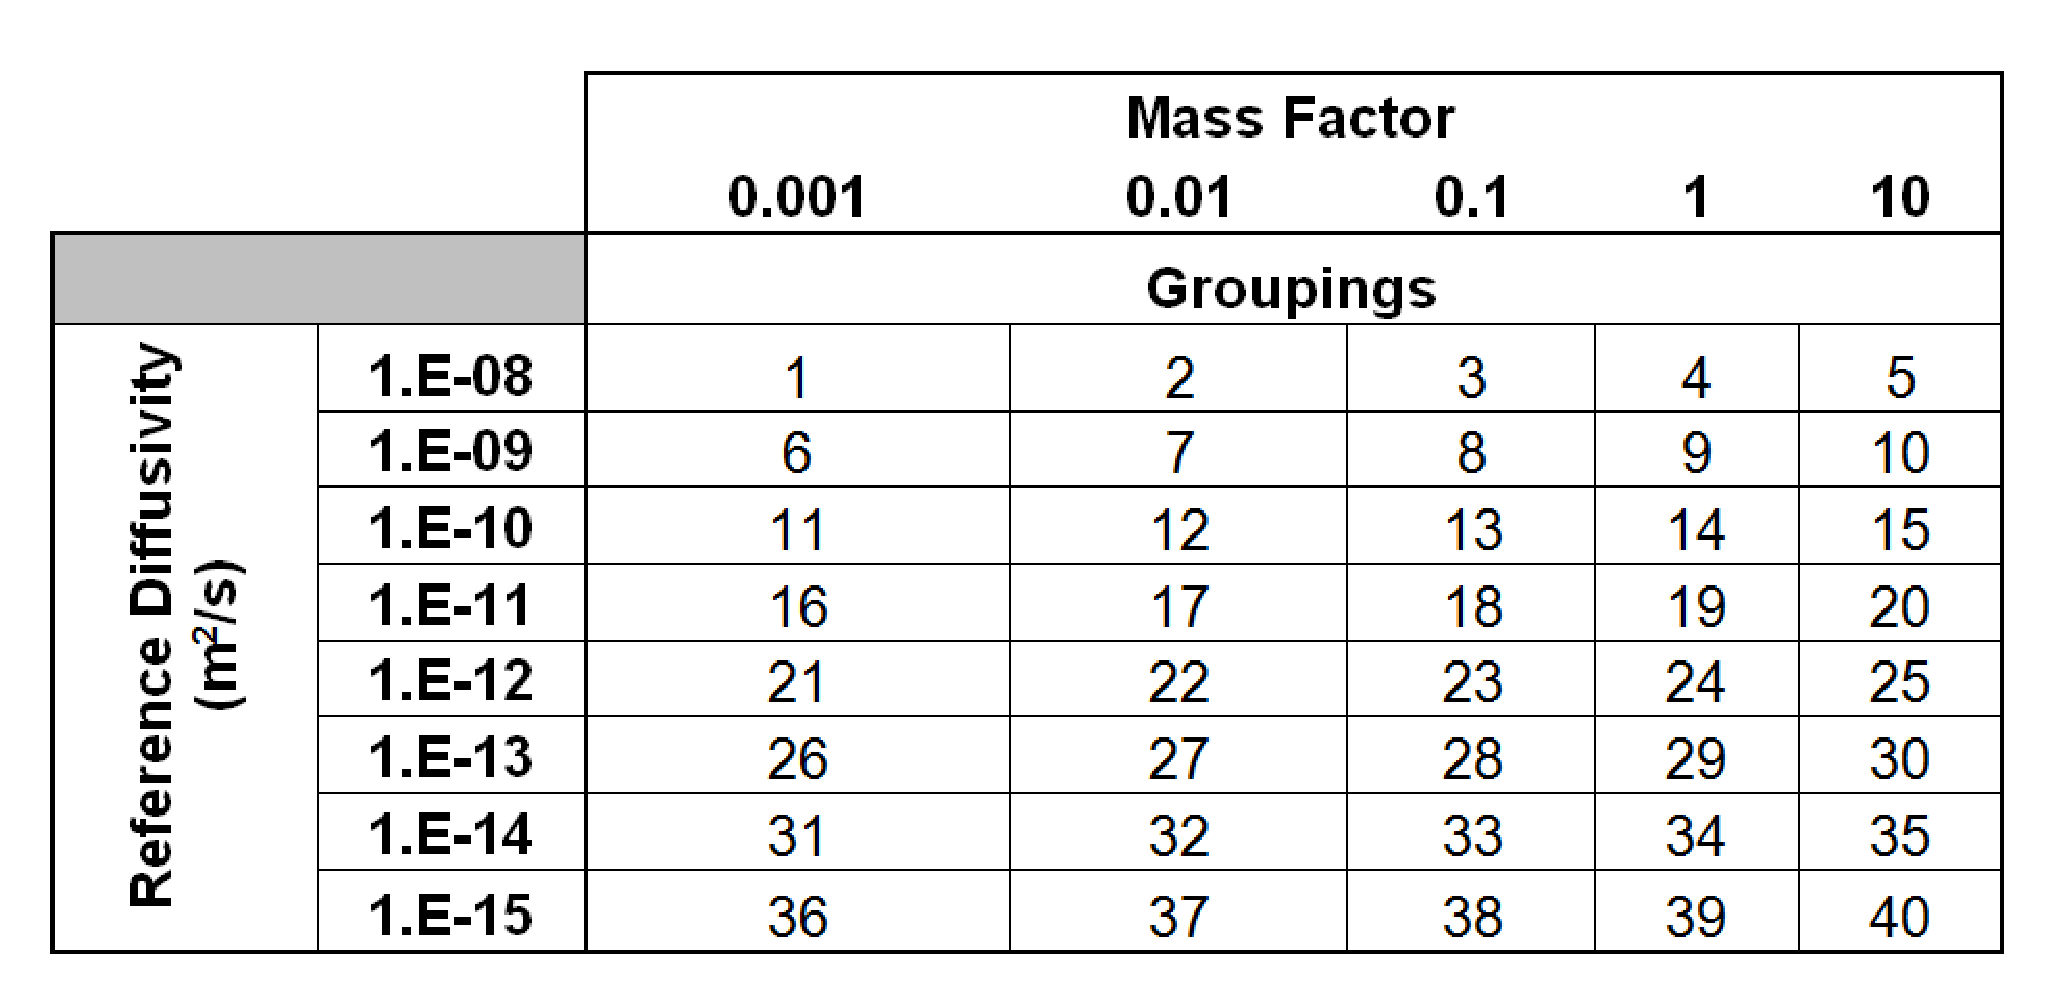
\includegraphics[width=0.8\textwidth]{DiffCoeffAndInvEBSFail/DiffCoeffAndInvGroups.eps}
\caption{Diffusion coefficient and mass factor simulation groupings.}
\label{tab:DiffCoeffAndInvGroups}
\end{table}
\end{frame}

\begin{frame}[c]
  \frametitle{Case I : Diffusion Coefficient and Inventory}
\begin{figure}[ht]
\centering
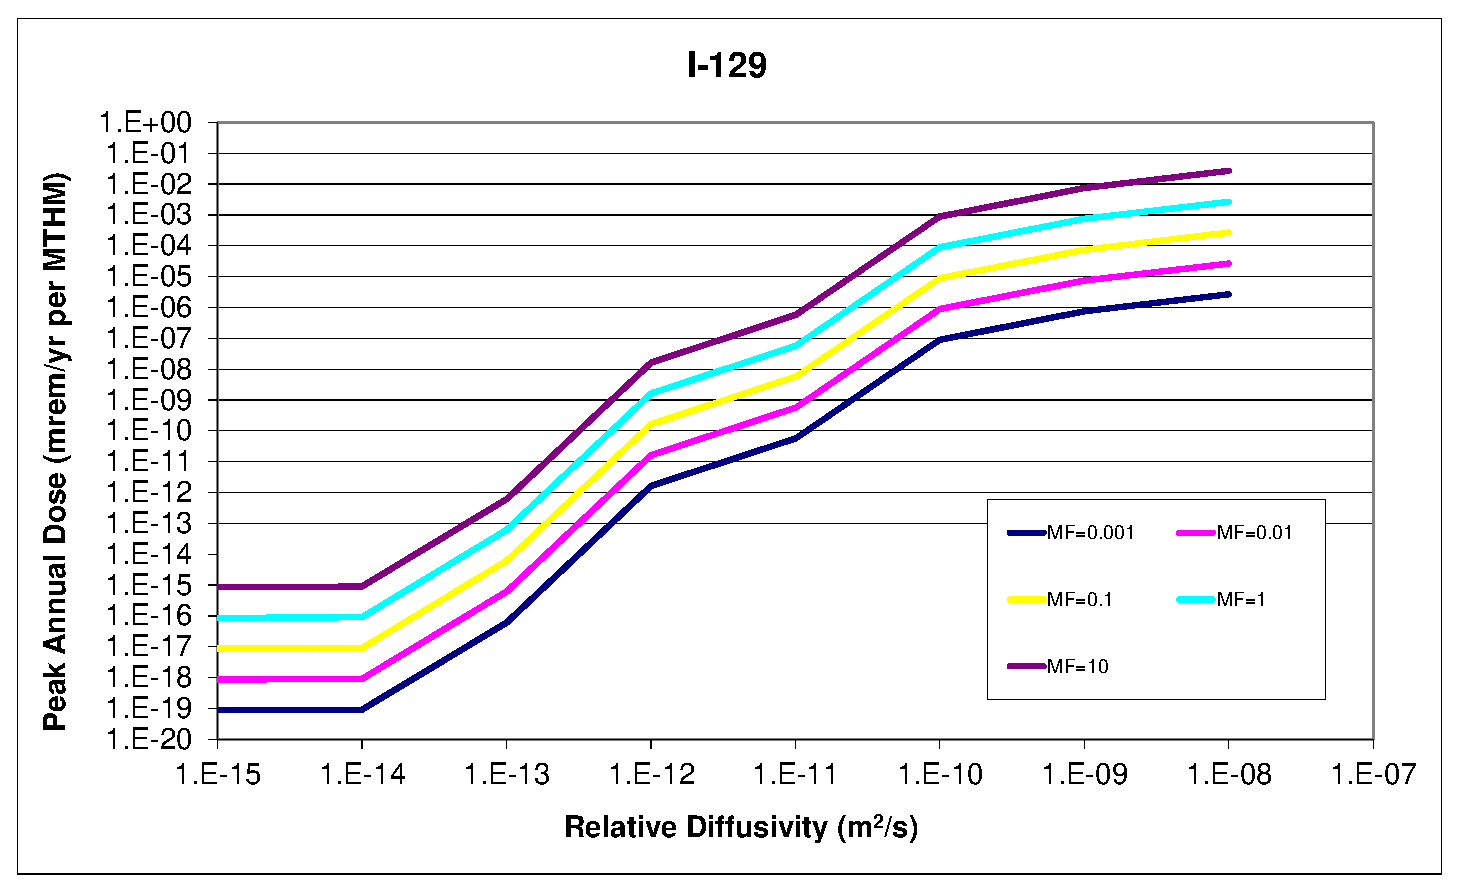
\includegraphics[width=0.8\textwidth]{./DiffCoeffAndInvEBSFail/I-129.eps}
\caption{The peak doses due to highly soluble, non-sorbing elements such as $I$ 
are largely directly proportional to the relative diffusivity.  }
\label{fig:DCInvI129}
\end{figure}
\end{frame}

\begin{frame}[c]
  \frametitle{Case I : Diffusion Coefficient and Inventory}
\begin{figure}[ht]
\centering
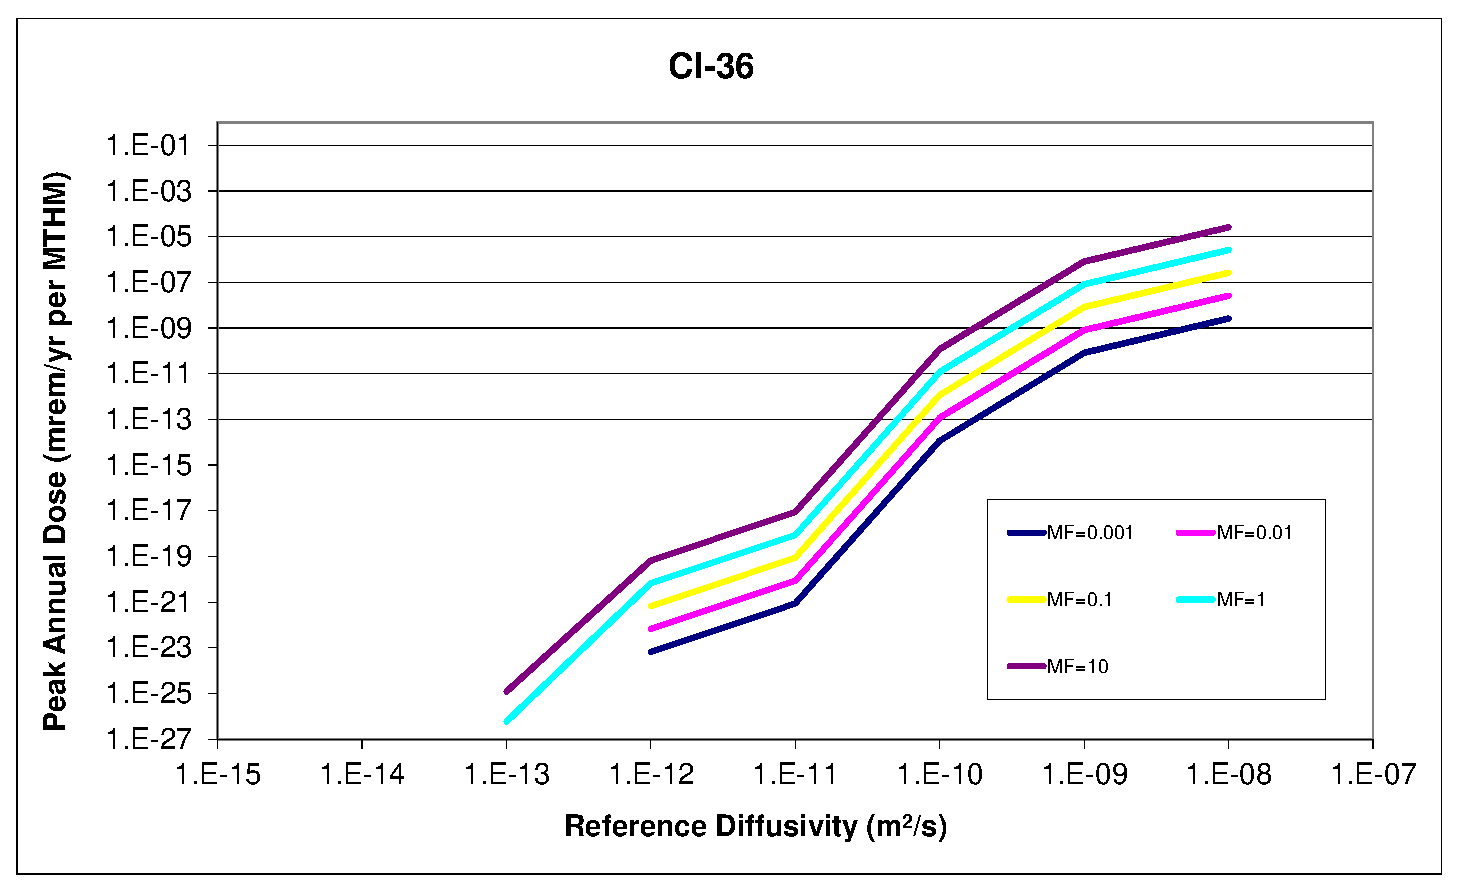
\includegraphics[width=0.8\textwidth]{DiffCoeffAndInvEBSFail/Cl-36.eps}
\caption{The peak doses due to highly soluble, non-sorbing elements such as $Cl$ 
are largely directly proportional to the relative diffusivity.  }
\label{fig:DCInvCl36}
\end{figure}
\end{frame}

\begin{frame}[c]
  \frametitle{Case I : Diffusion Coefficient and Inventory}
\begin{figure}[ht]
\centering
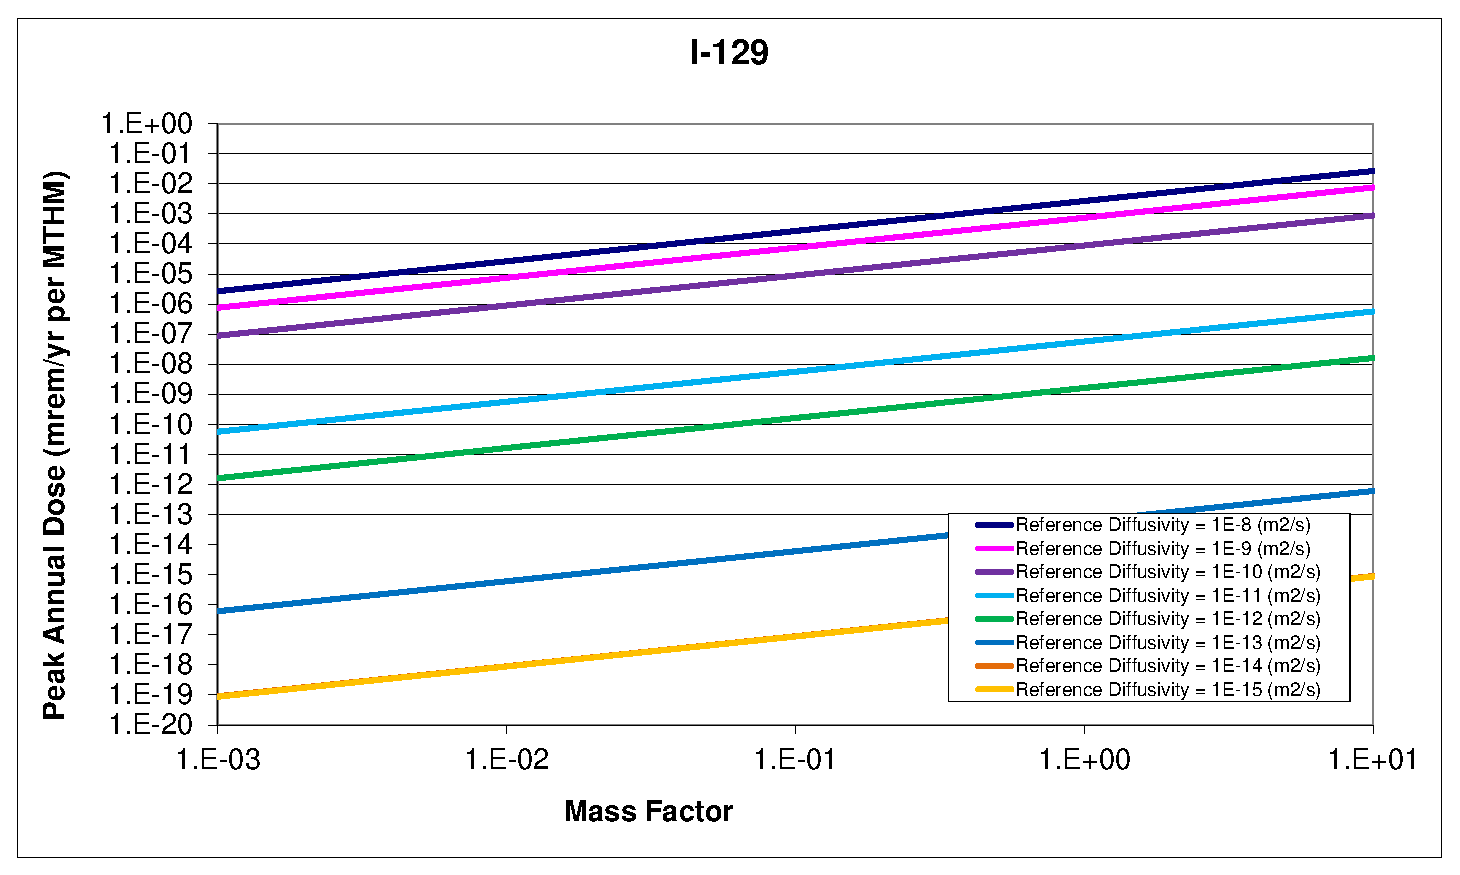
\includegraphics[width=0.8\textwidth]{DiffCoeffAndInvEBSFail/I-129-MF.eps}
\caption{The peak doses due to highly soluble, non-sorbing elements such as $I$ 
are  proportional to the radionuclide inventory.}
\label{fig:DCInvI129MF}
\end{figure}
\end{frame}

\begin{frame}[c]
  \frametitle{Case I : Diffusion Coefficient and Inventory}

\begin{figure}[ht]
\centering
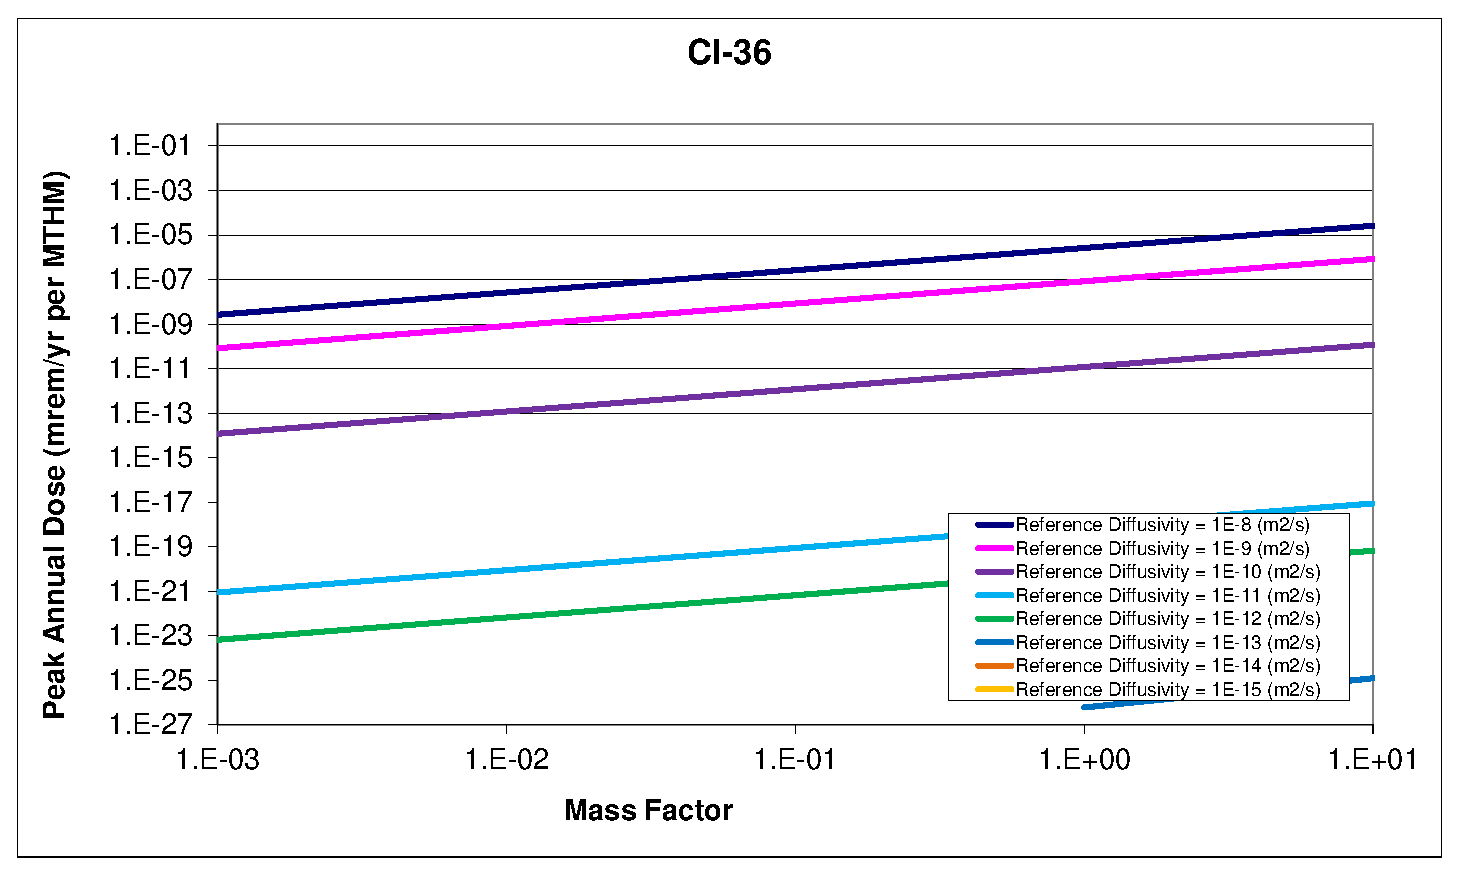
\includegraphics[width=0.8\textwidth]{DiffCoeffAndInvEBSFail/Cl-36-MF.eps}
\caption{The peak doses due to highly soluble, non-sorbing elements such as $I$ 
are  proportional to the radionuclide inventory.}
\label{fig:DCInvCl36MF}
\end{figure}
\end{frame}


\begin{frame}[c]
  \frametitle{Case I : Diffusion Coefficient and Inventory}
\begin{figure}[ht!]
\centering
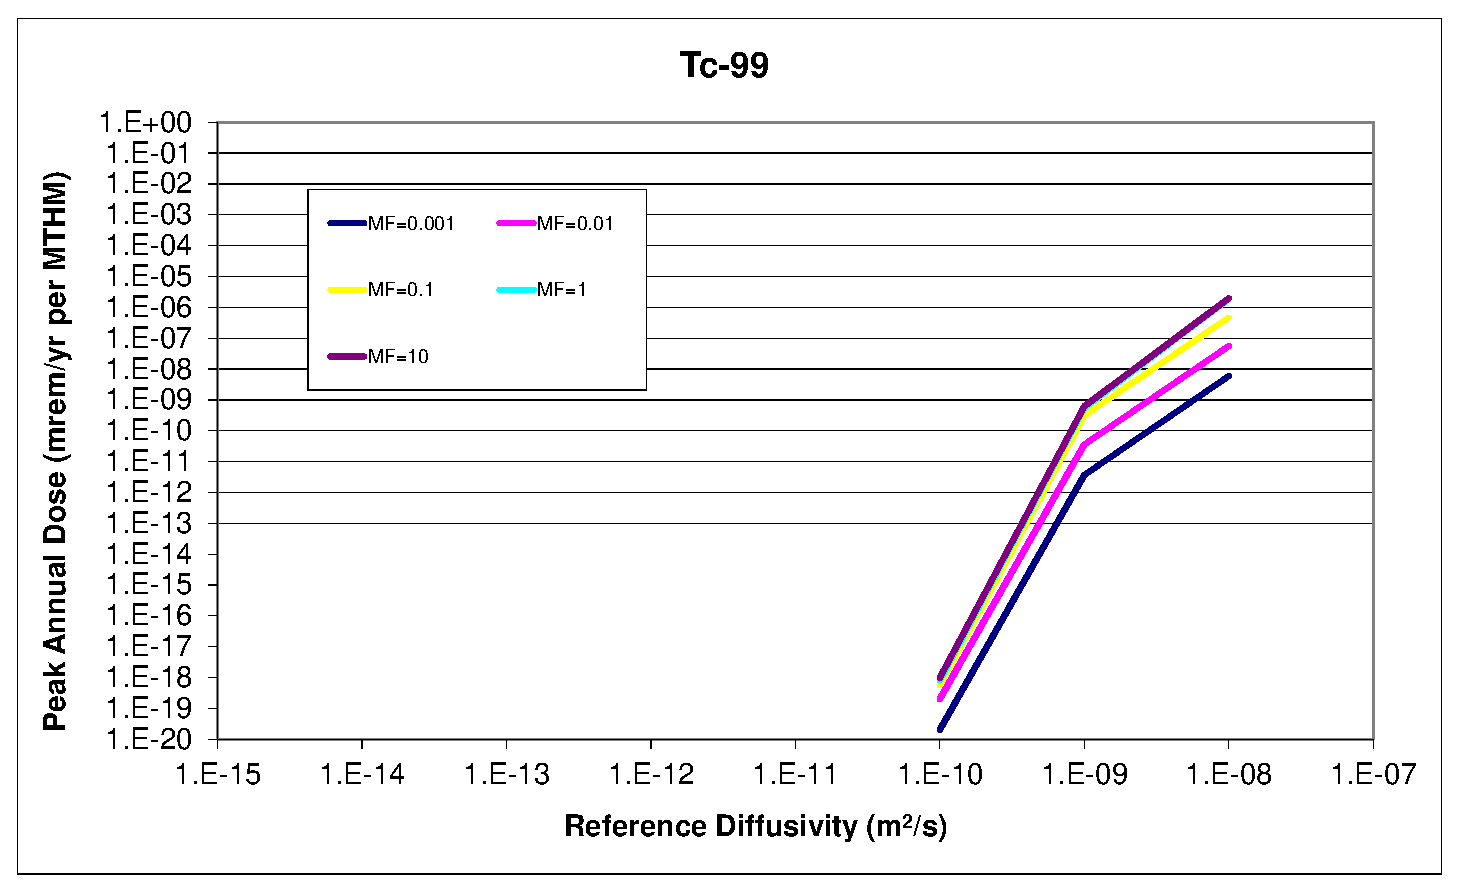
\includegraphics[width=0.8\textwidth]{DiffCoeffAndInvEBSFail/Tc-99.eps}
\caption{$^{99}Tc$ relative diffusivity sensitivity.} 
\label{fig:DCInvTc99}
\end{figure}
\end{frame}

\begin{frame}[c]
  \frametitle{Case I : Diffusion Coefficient and Inventory}
\begin{figure}[ht!]
\centering
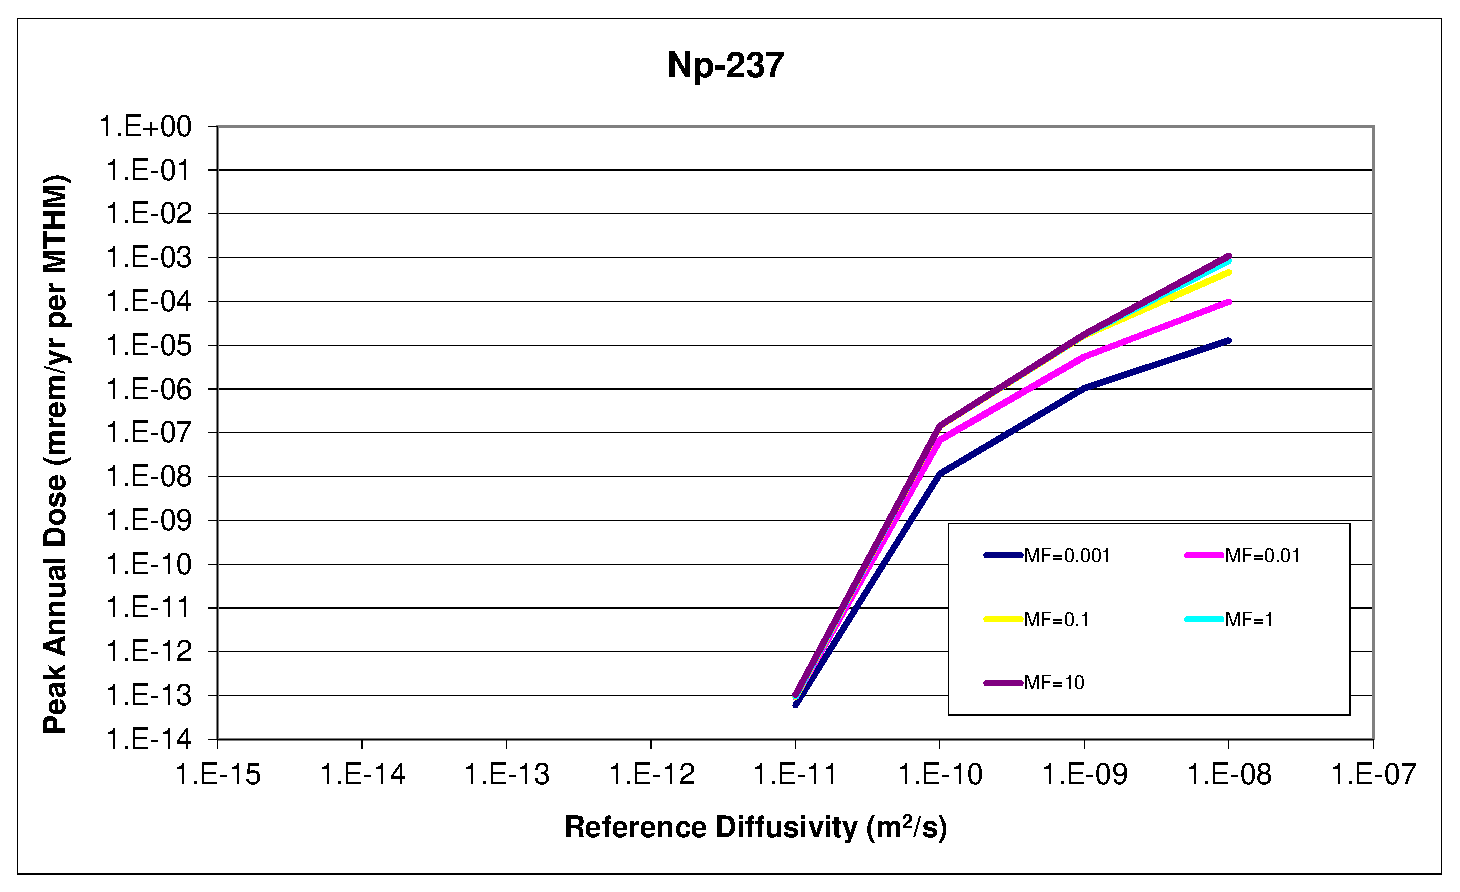
\includegraphics[width=0.8\textwidth]{DiffCoeffAndInvEBSFail/Np-237.eps}
\caption{$^{237}Np$ relative diffusivity sensitivity.} 
\label{fig:DCInvNp237}
\end{figure}
\end{frame}

\begin{frame}[c]
  \frametitle{Case I : Diffusion Coefficient and Inventory}

\begin{figure}[ht!]
\centering
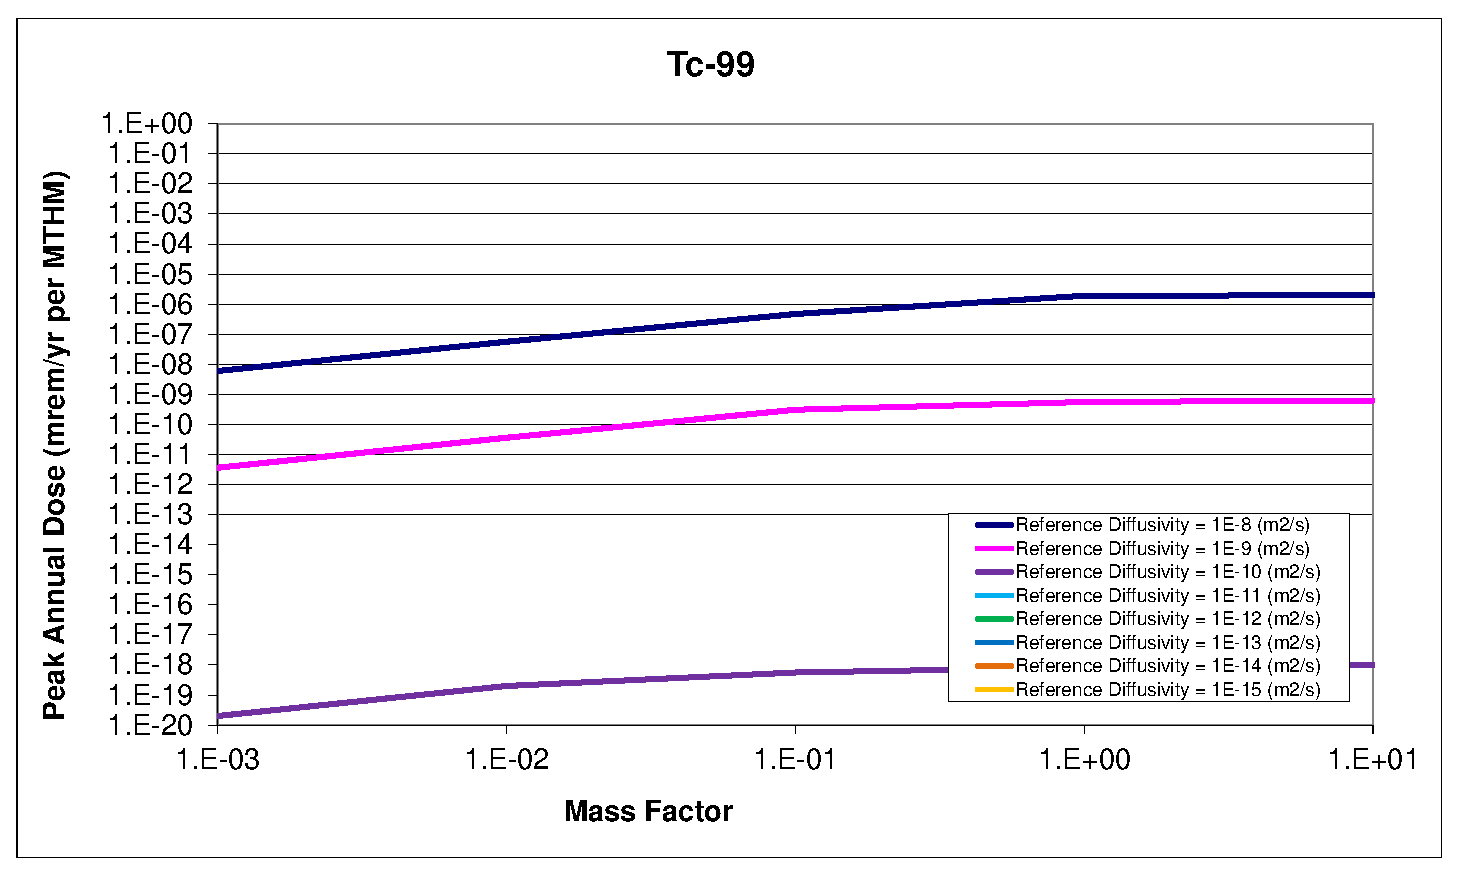
\includegraphics[width=0.8\textwidth]{DiffCoeffAndInvEBSFail/Tc-99-MF.eps}
\caption{$^{99}Tc$ mass factor sensitivity.}
\label{fig:DCInvTc99MF}
\end{figure}
\end{frame}

\begin{frame}[c]
  \frametitle{Case I : Diffusion Coefficient and Inventory}

\begin{figure}[ht!]
\centering
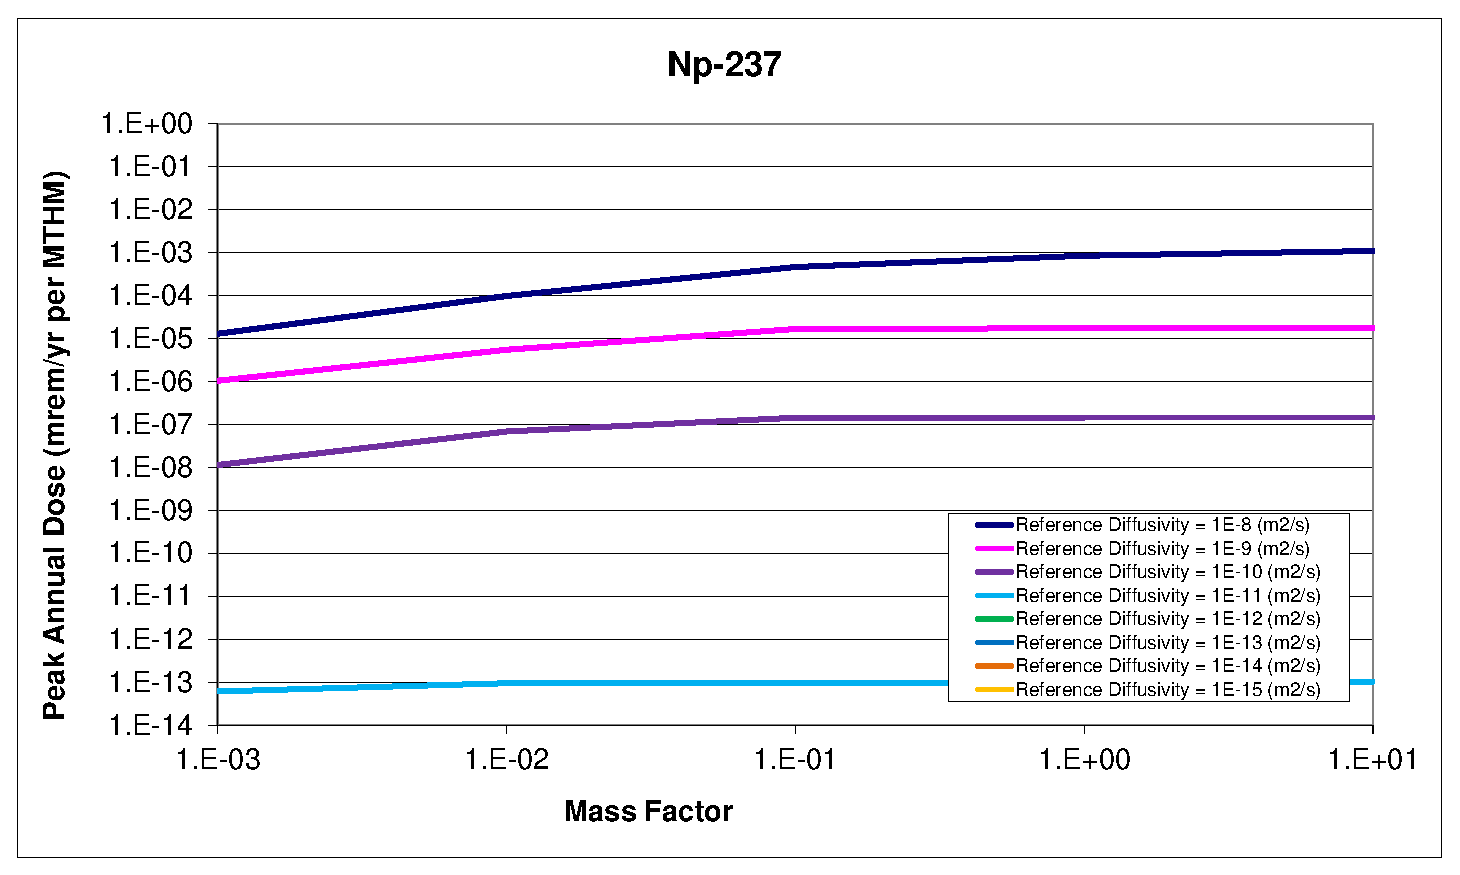
\includegraphics[width=0.8\textwidth]{DiffCoeffAndInvEBSFail/Np-237-MF.eps}
\caption{$^{237}Np$ mass factor sensitivity.}
\label{fig:DCInvNp237MF}
\end{figure}
\end{frame}
